\documentclass[12pt]{article}
\usepackage{amsmath}
\usepackage{fontspec}
\usepackage{xunicode}
\usepackage{xltxtra}
\setromanfont{FreeSerif}
\setsansfont{FreeSans}
\setmonofont{FreeMono}
\usepackage{caption}
\usepackage{subcaption}


\usepackage{geometry}
 \geometry{
 a4paper,
 total={210mm,297mm},
 left=20mm,
 right=20mm,
 top=20mm,
 bottom=20mm,
 }
 \usepackage{graphicx}
 \DeclareGraphicsExtensions{.pdf,.png,.jpg}
\usepackage{float}

\title{Groceries}
\author{Ευάγγελος Καραγεώργος - Βασίλιος Σκούρτης }
\date{}
\begin{document}
  \maketitle
  \section{Περιγραφή}
  	\paragraph{}
  	  Η εργασία είναι ένα λειτουργικό e-shop, που εμπορεύεται τρόφιμα και άλλα είδη παντοπωλείου.
  	  \par 
  \section{Βάση}
  	\subsection{E-R διάγραμμα}
		\begin{figure}[H]
			\centering
			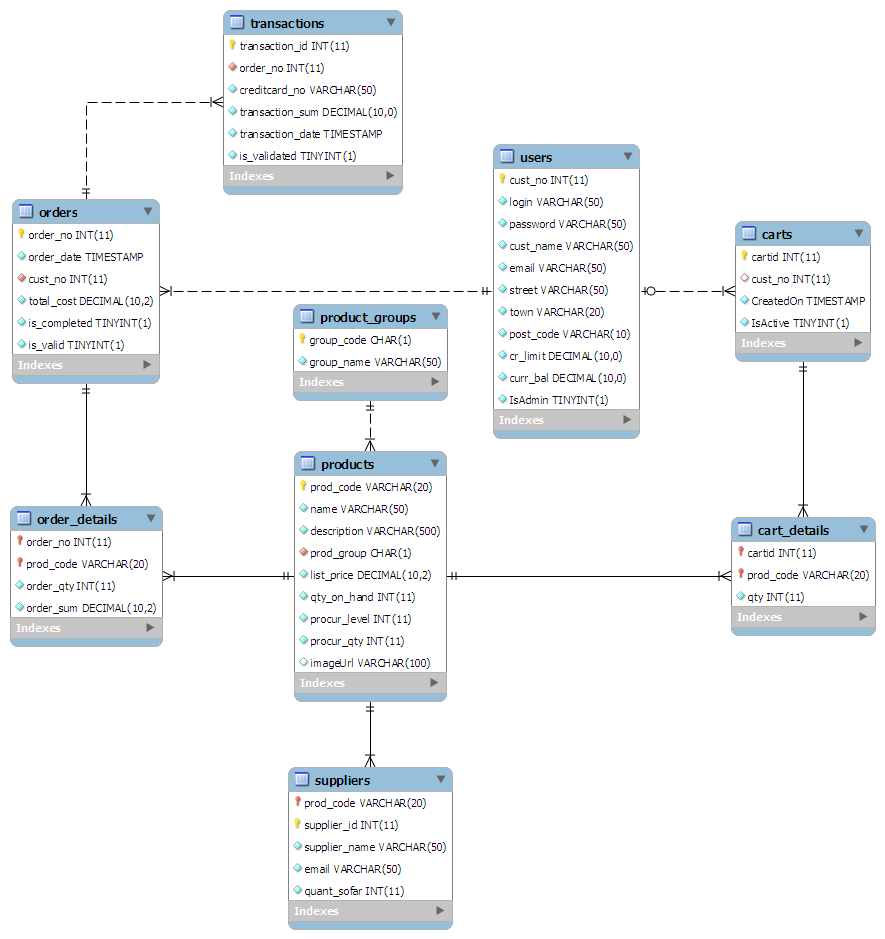
\includegraphics[width=1\textwidth]{ER_model}
			\caption{Groceries E-R model}
		\end{figure}
	\pagebreak
	\subsection{Functions και Procedures}
  	  \paragraph{}
  	  	Πολλές από τις βασικές λειτουργίες υλοποιούνται με τη βοήθεια κάποιων functions και procedures που φροντίζουν πολλές λειτουργίες να γίνονται atomic και με ασφάλεια:
  	  	\begin{itemize}
  	  		\item procedure user\_login (ilogin, ipassword) : Λαμβάνοντας ένα login name και ένα password, η διαδικασία ελέγχει τα στοιχεία και κάνει ενα select επιστρέφοντας ένα table με IsAuth, IsAdmin και cust\_no, που υποδηλώνουν εάν τα στοιχεία αντιστοιχούν σε χρήστη, εάν ο χρήστης είναι admin και ποιό είναι το cust\_no του χρήστη (-1 στην περίπτωση που τα στοιχεία είναι λάθος).
  	  		\item function user\_register (ilogin, ipass, ifullname, iemail, istreet, itown, ipostcode) : Εγγράφει έναν νέο χρήστη εάν το login name δεν υπάρχει ήδη. Επιστρέφει το cust\_no του χρήστη που προστέθηκε, αλλιώς -1.
  	  		\item function add\_to\_cart (icartid, iprod\_code, iqty) : Προσπαθεί να προσθέσει στο καλάθι με cartid = icartid, ποσότητα iqty από το προιόν με κωδικό iprod\_code. Η ποσότητα που προσθέτουμε μπορεί να είναι και αρνητική για να αφαιρέσουμε από το καλάθι. Η συνάρτηση ελέγχει και το stock του προϊόντος και κάνει τις απαραίτητες ριθμίσεις, ώστε να είναι συμβατή η τελική ποσότητα με το qty\_on\_hand του προιόντος. Επίσης, εάν το προϊόν καταλήξει να είναι με ποσότητα 0, αφαιρείται απ'τον πίνακα cart\_details εντελώς. Η συνάρτηση επιστρέφει την τελική διαφορά ποσότητας σε σχέση με την προηγούμενη ποσότητα που είχε το προϊόν.
  	  		\item procedure get\_cart (icartid) : Η διαδικασία κανονικοποιεί ολόκληρο το καλάθι με cartid-icartid, όσον αφορά τις΅ποσότητες των προϊόντων και το qty\_on\_hand τους, πιθανόν και αφαιρώντας αυτά που δεν έχουν stock καθόλου, και κάνει ένα select με όλα τα δεδομένα του καλαθιού.
  	  		\item function convert\_cart\_to\_order (icartid) : Μετατρέπει ένακαλάθι σε παρραγελία. Εάν το καλάθι δεν υπάρχει ή είναι ανενεργό ή ο χρήστης που αντιστοιχεί στο καλάθι δεν έχει αρκετό cr\_limit-curr\_bal για να χρεωθεί την παραγγελία, η συνάρτηση επιστρέφει αρνητικό αριθμό που αντιστοιχεί στην αποτυχία. Αλλιώς, η συνάρτηση κάνει normalize το καλάθι, φτιάχνει μία παραγγελία, την ορίζει να περιέχει τα περιεχόμενα του καλαθιού, ορίζει το καλάθι ως ανενεργό, προσθέτει στο curr\_bal του χρήστη το ποσό της παραγγελίας, αφαιρεί τις΅ποσότητες των προϊόντων απο το qty\_on\_hand τους και επιστρέφει τον αριθμό παραγγελίας που δημιουργήθηκε.
  	  		\item procedure create\_transaction (iorder\_no, icretidcard\_no) : Δημιουργεί μία συναλλαγή πληρωμής για μία παραγγελία με έναν συγκεκριμένο αριθμό πιστωτικής κάρτας. Το ποσό συναλλαγής ορίζεται αυτό του κόστους της παραγγελίας.
  	  		\item procedure cancel\_order (iorder\_no) : Ακυρώνει μία εν'εξελίξει παραγγελία με το να την ορίζει ως΅άκυρη και να επιστρέφει τις ποσότητες των προϊόντων στα αντίστοιχα qty\_on\_hand.
  	  		\item function complete\_order (iorder\_no) : Εφόσον ελέγξει ότι η παραγγελία υπάρχει, είναι εν'εξελίξει και υπάρχει το αντίστοιχο transaction με το ποσό, ορίζει την παραγγελία ως ολοκληρωμένη και επιστρέφει 1. Σε περίπτωση αποτυχίας επιστρέφει 0.
  	  		\item function supply\_produc\_new\_supplier (iprod\_code, isuppliername, isupplieremail) : Εάν το όνομα προμηθευτή υπάρχει ήδη επιστρέφει -1, αλλίώς δημιουργεί νέο προμηθευτή με τα στοιχεία για το προϊόν (και το σωστό quant\_sofar ανάλογαα με το procur\_qty), πεοσθέτει στο qty\_on\_hand to procur\_qty του προϊόντος και επιστρέφει το supplier\_id που δημιουργήθηκε.
  	  		\item procedure supply\_product (iprod\_code, isupplier\_id) : Προμηθεύει το προϊόν από τον συγκεκριμένο προμηθευτή κάνοντας τα κατάλληλα adjustments σε qty\_on\_hand, quant\_sofar και προσθέτοντας την κατάλληλη εγγραφή στον πίνακα suppliers εάν δεν υπάρχει ήδη.
  	  	\end{itemize}
  	\subsection{Queries}
  	  \paragraph{}
  	  	 	 	
\end{document}